\documentclass[9pt,twocolumn,twoside]{pnas-new}
% Use the lineno option to display guide line numbers if required.
% Note that the use of elements such as single-column equations
% may affect the guide line number alignment. 

\templatetype{pnasresearcharticle} % Choose template 
% {pnasresearcharticle} = Template for a two-column research article
% {pnasmathematics} = Template for a one-column mathematics article
% {pnasinvited} = Template for a PNAS invited submission

\title{Which Findings from the Functional Neuroimaging Literature Can We Trust?}



\newcommand{\subtext}[2]{
#1_{_{\text{#2}}}
}



\author[a,1,2]{Daniel Kessler}
\author[a,1]{Michael Angstadt} 
\author[a,1]{Chandra Sripada}

\affil[a]{Department of Psychiatry, University of Michigan, Ann Arbor}

\leadauthor{Kessler}

% Please add here a significance statement to explain the relevance of your work
% \significancestatement{Authors must submit a 120-word maximum statement about the significance of their research paper written at a level understandable to an undergraduate educated scientist outside their field of speciality. The primary goal of the Significance Statement is to explain the relevance of the work in broad context to a broad readership. The Significance Statement appears in the paper itself and is required for all research papers.}

% Please include corresponding author, author contribution and author declaration information
\authorcontributions{DK, MA, and CS planned and executed the analysis and wrote the letter.}
\authordeclaration{The authors have no conflicts of interest to declare.}
\equalauthors{\textsuperscript{1}All authors contributed equally to this work.}
\correspondingauthor{\textsuperscript{2}To whom correspondence should be addressed. E-mail: kesslerd@umich.edu}

% Keywords are not mandatory, but authors are strongly encouraged to provide them. If provided, please include two to five keywords, separated by the pipe symbol, e.g:
%\keywords{Keyword 1 $|$ Keyword 2 $|$ Keyword 3 $|$ ...} 

\begin{abstract}
In their recent ``Cluster Failure'' paper, Eklund and colleagues \cite{eklund_cluster_2016} cast doubt on the accuracy of a widely used statistical test in functional neuroimaging. 
Here, we leverage nonparametric methods that control the false discovery rate in order to offer more nuanced, quantitative guidance about which findings in the existing literature can be trusted. 
We show that, in the task studies examined by Eklund et al., most clusters originally reported to be significant are indeed trustworthy by the false discovery rate benchmark.
\end{abstract}


\dates{This manuscript was compiled on \today}
\doi{\url{www.pnas.org/cgi/doi/10.1073/pnas.XXXXXXXXXX}}

\begin{document}

% Optional adjustment to line up main text (after abstract) of first page with line numbers, when using both lineno and twocolumn options.
% You should only change this length when you've finalised the article contents.
\verticaladjustment{-2pt}

\maketitle
\thispagestyle{firststyle}
\ifthenelse{\boolean{shortarticle}}{\ifthenelse{\boolean{singlecolumn}}{\abscontentformatted}{\abscontent}}{}




% If your first paragraph (i.e. with the \dropcap) contains a list environment (quote, quotation, theorem, definition, enumerate, itemize...), the line after the list may have some extra indentation. If this is the case, add \parshape=0 to the end of the list environment.
\dropcap{I}n a substantial contribution to the functional magnetic resonance imaging (fMRI) field, Eklund et al. \cite{eklund_cluster_2016} use nonparametric methods to demonstrate that random field theory (RFT)-based family-wise error (FWE) correction techniques for cluster-level inference do not control errors as they are supposed to, and this discrepancy is pronounced for lenient cluster defining thresholds (CDT). 
Moreover, they point to violations of RFT assumptions as the culprit for this discrepancy.

Given these results, what advice can we offer to the reader exploring existing fMRI literature when faced with a table of cluster-wise RFT-based FWE-corrected \textit{p}-values ($\subtext{p}{RFT-FWE}$)? 
To suggest caution is reasonable but incomplete; we require concrete, quantitative guidelines to enable appropriate calibration of skepticism.

Here, we undertake an initial attempt to construct such guidance.
We heed Eklund et al.'s warning and prefer null distributions obtained through nonparametric methods rather than RFT.
However, we focus on the False Discovery Rate (FDR; \cite{benjamini_controlling_1995}), which is a more natural target for multiple testing control (as recognized by Nichols in previous work; \cite{genovese_thresholding_2002}):
A researcher is naturally more concerned with the proportion of reported clusters that are false positives (FDR) than whether \textit{any} are false positives (FWE).
Given these considerations, a reader faced with a table of clusters significant under RFT-FWE correction might ask: Which of these results would have survived had the study instead employed a nonparametric FDR-based method?

We address this question using task fMRI data \cite{duncan_consistency_2009,tom_neural_2007} analyzed by Eklund et al. (available from openfMRI \cite{poldrack_toward_2013}).

For each contrast, we generate 5,000 realizations of the data through sign-flipping (our code, data, Extended Methods: \url{http://github.com/mangstad/FDR_permutations}).
To obtain a null distribution of cluster extents (for an arbitrarily chosen cluster), we combine normalized frequencies of extents at each realization.
This distribution is used to assign uncorrected \textit{p}-values to each observed cluster. 
We next submit the vector of uncorrected \textit{p}-values for each contrast to Benjamini and Hochberg's \cite{benjamini_controlling_1995} FDR procedure with $\subtext{\alpha}{FDR}=.05$ (cf. \cite{chumbley_false_2009} for a parametric implementation of cluster-wise FDR).
 
We compare $\subtext{p}{RFT-FWE}$-values to $\subtext{q}{FDR}$-values and note whether they survive FDR-correction under $\subtext{\alpha}{FDR}=.05$. 
We generate separate plots for this analysis conducted at CDT=\{.001, .01\}.

\begin{figure*}[ht]
\IfFileExists{../Results/FDR_surviving_clusters.pdf}{\includegraphics[width=1.0\textwidth]{../Results/FDR_surviving_clusters.pdf}}{\includegraphics[width=1.0\textwidth]{FDR_surviving_clusters.pdf}}
\centering
\caption{
\textbf{Assessing RFT-Based FWE Using an FDR Benchmark.}
We submitted the same task data analyzed by Eklund et al. \cite{eklund_cluster_2016,tom_neural_2007,poldrack_toward_2013} to nonparametric clusterwise FDR analysis. For $\text{CDT}=.001$ (top), RFT-based FWE approximates effective FDR control with $\subtext{\alpha}{FDR} = .05$. For $\text{CDT}=.01$ (bottom), only clusters with $\subtext{p}{RFT-FWE} \leq .00001$ reliably survived correction at $\subtext{\alpha}{FDR}=.05$. 
\label{fig:p-plot}
}
\end{figure*}

Results (see Figure \ref{fig:p-plot}) show that for CDT=.001, only one cluster significant at $\subtext{\alpha}{RFT-FWE} = .05$ failed to survive at $\subtext{\alpha}{FDR} = .05$, thus suggesting RFT-based FWE closely approximates effective FDR control.
This finding has promising implications for past fMRI studies using RFT-based cluster-level inference that used this stricter CDT, estimated to be upwards of 8,500 reports \cite{nichols_bibliometrics_2016,woo_cluster-extent_2014}.
For CDT=.01, used in approximately 3,500 studies \cite{nichols_bibliometrics_2016,woo_cluster-extent_2014}, Eklund et al. and others \cite{flandin_analysis_2016} have urged caution and our results agree. We found that $\subtext{\alpha}{RFT-FWE}$ must be very strict for effective FDR control (i.e., many $.00001 \leq \subtext{p}{RFT-FWE} \leq .05$ fail to survive correction at $\subtext{\alpha}{FDR}=.05$).


These results offer initial guidance on interpreting past literature that employed RFT-based FWE, providing a more granular appreciation of the relationship between $\subtext{p}{RFT-FWE}$ and trustworthiness of the result.
A more comprehensive examination of fMRI task data sets that used RFT-based FWE may further refine this guidance.

\acknow{We thank Anders Eklund and Thomas Nichols for providing us with processed data and for very helpful comments on earlier versions of this letter.}

\showacknow % Display the acknowledgments section

\pnasbreak

\bibliography{biblio}


\end{document}
